% Provenance (never printed): see sources/outline_sources.md (Year 3: gravity, magnetic,
% seismic, resistivity and ground-penetrating-radar surveys; data processing and
% uncertainty; a mapping project).
% Brief: sources/book5/BRIEFS.md, ch. 31. Curves from figdata/bachelor-3/gravity_granite.py
% (prism model of the Varden granite of figdata/shared/region.py), magnetic_dyke.py (2-D
% dyke; the Varden dolerite dyke of the Sync 3 ruling, buried below the unconformity),
% resistivity_sounding.py (Pekeris transform and image series) and gpr_radargram.py.
% Physical-property ranges and survey practice from the GPG open textbook (CC BY 4.0) and
% Keys (1990). Exercise and problem values in the Book 5 scratch calculator calc/ch31.py.
\chapter{Méthodes de terrain et de laboratoire III}\label{ch:b3:field-lab-methods-3}

Une équipe de géophysiciens passe une semaine dans la vallée des Varden Hills, la
région fictive dont le volume de première année a dressé la carte géologique, dans son
chapitre consacré aux cartes géologiques. La carte montre un granite affleurant sur les
flancs de la vallée, entre les schistes, sous le grès qui repose sur les deux. Là où le
granite disparaît sous la couverture, on ignore jusqu'où il s'étend et à quelle
profondeur il descend. L'équipe emporte un gravimètre, deux magnétomètres, un câble
d'électrodes et un \omterm{def:b3:field-lab-methods-3:gpr}{géoradar} monté sur un petit chariot. Aucun de ces instruments ne voit
une roche~: chacun mesure un champ en surface---la pesanteur, le champ magnétique, un
potentiel électrique, l'écho d'une impulsion radio---que les roches du sous-sol
perturbent. Au terme de la semaine, l'équipe peut dessiner le granite qu'elle n'a jamais
vu, dire quelle est la profondeur des alluvions du fond de vallée,
et signaler un corps magnétique
qu'aucune carte ne montrait.

Ce chapitre suit cette semaine. Il traite chaque méthode tour à tour, comme une mesure
assortie de ses corrections, et comme un \omterm{def:b3:seismology-imaging:inverse}{problème direct} portant sur quelques corps
dont les champs se calculent exactement~; il expose ensuite comment se cumulent les erreurs
d'une campagne et pourquoi un seul type de données fixe rarement un modèle~; il se termine
par la campagne de Varden, où les méthodes sont mises
en œuvre ensemble.

\begin{recall}
L'anomalie de pesanteur, les corrections et anomalies à l'air libre et de Bouguer, ainsi que la
pesanteur normale, figurent dans le volume de première année, dans son chapitre sur l'isostasie
et la gravité~; la boucle de mesure d'un \omterm{def:b3:field-lab-methods-3:gravimeter}{gravimètre relatif} est décrite au
\cref{ch:b3:gravity-geodesy}. Le champ principal, son inclinaison, la \omterm{thm:b3:palaeomagnetism:dipole}{formule du dipôle} et
le \omterm{def:b3:palaeomagnetism:igrf}{champ géomagnétique international de référence} (IGRF) sont traités au
\cref{ch:b3:palaeomagnetism}. La résistivité, la loi d'Ohm, la permittivité relative, les ondes
électromagnétiques, l'aimantation et la susceptibilité magnétique relèvent des volumes de physique,
de même que le théorème de Gauss pour la gravité. Les \omterm{def:b3:exploration-seismology:surveys}{campagnes de sismique réfraction} sont
traitées au \cref{ch:b3:exploration-seismology}~; le \omterm{def:b3:seismology-imaging:inverse}{problème direct}, le \omterm{def:b3:seismology-imaging:inverse}{problème inverse}
et les moindres carrés pondérés sont traités au \cref{ch:b3:seismology-imaging}~; la porosité
figure dans les manuels du secondaire, et les \omterm{def:b3:facies-models:wireline}{diagraphies} au \cref{ch:b3:facies-models}.
La propagation des incertitudes est traitée dans les volumes de chimie
et de mathématiques.
\end{recall}

\section{Campagnes gravimétriques}\label{sec:b3:field-lab-methods-3:gravity}

Les anomalies recherchées par une campagne gravimétrique sont faibles. La pesanteur à
l'équateur vaut environ \qty{978000}{\milli\gal}~; les grandes structures la modifient
de plusieurs centaines de milligals, un dôme de sel d'une dizaine,
un corps minéralisé d'environ un, et les cibles d'une campagne
géotechnique de quelques centièmes. Les géophysiciens mesurent en milligals,
ou en unités de \qty{0.1}{\milli\gal}~; une campagne utile doit résoudre
des écarts d'une partie sur cent millions de~$g$.
% ledger: gpg:grav-units, gpg:grav-sizes

\begin{definition}[Gravimètre relatif~; dérive instrumentale]\label{def:b3:field-lab-methods-3:gravimeter}
Un \emph{gravimètre relatif}\index{gravimètre relatif} est un instrument qui mesure des
écarts de pesanteur entre stations~: une masse suspendue à un ressort, maintenue
en position nulle par une seconde force réglable. La lecture du cadran de cette force,
multipliée par une constante d'étalonnage, donne la pesanteur en milligals à une constante
inconnue près. Sa \emph{dérive instrumentale}\index{dérive instrumentale} est la lente
variation de sa lecture en un point fixe,
due au fluage du ressort, à la température et aux chocs~; on la mesure en relisant, après
quelques heures, une station déjà lue, la
\emph{station de base}.
\end{definition}
% ledger: gpg:gravimeter, gpg:grav-survey

Un gravimètre de terrain couvre une plage de plusieurs dizaines de milliers de
milligals et se lit, au mieux, à environ \qty{0.01}{\milli\gal}~; la plage doit être
recalée après le transport. À cette précision, la hauteur de chaque station
compte autant que sa lecture~: une erreur de \qty{3.3}{cm} sur la hauteur fausse
\qty{0.01}{\milli\gal}, si bien que les positions sont relevées au moyen de récepteurs
satellitaires ou d'un niveau, au centimètre près. La station de base est réoccupée
toutes les deux heures environ. La marée terrestre, qui peut atteindre
\qty{0.3}{\milli\gal}, varie assez lentement sur ces heures pour pouvoir être éliminée
avec la dérive.
% ledger: gpg:gravimeter, gpg:grav-survey, gpg:grav-sizes

\begin{method}[Réduction d'une boucle gravimétrique]\label{met:b3:field-lab-methods-3:loop}
Une boucle part et revient à une station de base, lue aux instants $t_0$ et $t_1$.
\begin{enumerate}
  \item Calculer la vitesse de dérive $(r_1 - r_0)/(t_1 - t_0)$ à partir des deux
        lectures de la station de base~; elle inclut la marée.
  \item Retrancher de chaque lecture la dérive accumulée depuis $t_0$,
        $r - (t - t_0)(r_1 - r_0)/(t_1 - t_0)$, puis retrancher la lecture de base~:
        ce résultat est la pesanteur relative à la station de base.
  \item Corriger de la hauteur $\Delta h$ de la station au-dessus de la station de base~:
        ajouter la correction à l'air libre $\qty{0.3086}{\milli\gal.m^{-1}}
        \times\Delta h$ et retrancher la correction de Bouguer
        $\qty{0.1119}{\milli\gal.m^{-1}}\times\Delta h$ (masse volumique
        \qty{2670}{kg.m^{-3}}), soit ajouter $0.1967\,\Delta h$.
  \item Pour une station située à une distance $\Delta y$ au nord de la base, retrancher
        la variation de la pesanteur normale, $\qty{0.811}{\milli\gal.km^{-1}}
        \times\sin 2\varphi\times\Delta y$.
  \item Ajouter la \omterm{def:b3:field-lab-methods-3:terrain}{correction de terrain} de chaque station.
\end{enumerate}
Le résultat est l'anomalie de Bouguer relative à la base. Le rattachement de la base
à une station de pesanteur absolue connue donne l'anomalie elle-même.
\end{method}
% ledger: gpg:grav-survey, gpg:terrain

La correction de Bouguer traite le terrain compris entre la station et le
niveau de référence comme une dalle plane. Dans un relief réel, cette hypothèse est fausse à deux titres~:
une colline qui s'élève au-dessus de la station tire vers le haut et abaisse la
lecture, et une vallée qui s'enfonce sous elle est comptée dans la dalle comme
de la roche qui n'est pas là.

\begin{definition}[Correction de terrain]\label{def:b3:field-lab-methods-3:terrain}
La \emph{correction de terrain}\index{correction de terrain} d'une station de
pesanteur est l'attraction que les écarts du relief par rapport à la
dalle de Bouguer exercent sur elle~: les collines au-dessus du niveau de la station, et
les vallées au-dessous, comptées avec la masse volumique de la dalle. Les deux abaissent la
pesanteur mesurée par rapport à la dalle~; la correction est donc
toujours ajoutée.
\end{definition}

Elle a été calculée à la main, à l'aide d'un abaque de Hammer et de tables, zone par zone
en s'éloignant de la station~; elle l'est aujourd'hui à partir
d'un modèle numérique de terrain. Loin des reliefs abrupts, elle dépasse rarement \qty{1}{\milli\gal},
mais les zones proches de la station sont difficiles à calculer correctement, et la
correction n'est guère connue à mieux que \qty{0.2}{\milli\gal}.
% ledger: gpg:terrain, gpg:grav-sizes

\subsection{Anomalies de corps simples}

Le \omterm{def:b3:seismology-imaging:inverse}{problème direct} de la pesanteur est une somme~: chaque élément d'un corps de
contraste de masse volumique $\Delta\rho$ attire la station selon la loi de Newton, et
une campagne mesure la composante verticale de la somme. Quelques corps la donnent
sous forme fermée.

\begin{theorem}[Sphère et cylindre horizontal]\label{thm:b3:field-lab-methods-3:sphere}
À une distance horizontale $x$ du point situé à la verticale de son centre, une sphère
enfouie d'excès de masse $\Delta m$ dont le centre est à la profondeur $z$
donne l'anomalie
\[
\Delta g(x) = \frac{G\,\Delta m\,z}{(x^2 + z^2)^{3/2}} ,
\]
et l'anomalie tombe à la moitié de son maximum en $x_{1/2} = z\sqrt{2^{2/3} - 1}$,
de sorte que $z = 1.305\,x_{1/2}$. Un long cylindre horizontal d'excès de masse
$\lambda$ par unité de longueur, dont l'axe est à la profondeur $z$, donne en travers
de sa direction
\[
\Delta g(x) = \frac{2G\lambda z}{x^2 + z^2} ,
\]
et $z = x_{1/2}$.
\end{theorem}

\begin{proof}
Hors d'une sphère dont la masse volumique ne dépend que de la distance à son
centre, l'attraction est celle de sa masse placée au centre (le
théorème de la coque, conséquence du théorème de Gauss). Son intensité à la
station vaut $G\Delta m/(x^2 + z^2)$, et la composante verticale porte
le facteur $z/\sqrt{x^2 + z^2}$. En écrivant $\Delta g(x_{1/2}) =
\Delta g(0)/2$ on obtient $(1 + x_{1/2}^2/z^2)^{3/2} = 2$, d'où la règle. Pour
le cylindre, le théorème de Gauss sur un cylindre coaxial de rayon $r$ donne
un champ $2G\lambda/r$, et la composante verticale $2G\lambda z/r^2$~;
on atteint la moitié du maximum lorsque $x^2 + z^2 = 2z^2$.
\end{proof}
% ledger: gpg:half-width

Un corps qui n'est pas une sphère possède tout de même une demi-largeur, et la règle
donne alors la profondeur d'une sphère équivalente, et non celle du corps. La règle est
une première estimation, faite avant tout ajustement d'un modèle.

\begin{proposition}[Cylindre vertical sur son axe]\label{prop:b3:field-lab-methods-3:vcyl}
Un cylindre vertical de rayon $a$ et de contraste de masse volumique $\Delta\rho$,
dont le sommet et la base sont aux profondeurs $z_1 < z_2$ sous la station,
donne sur son axe
\[
\Delta g = 2\pi G\Delta\rho\left[(z_2 - z_1) + \sqrt{z_1^2 + a^2}
           - \sqrt{z_2^2 + a^2}\right] .
\]
Pour $a \to \infty$, c'est la dalle de Bouguer $2\pi G\Delta\rho(z_2 - z_1)$~;
pour un cylindre allant de la surface à une grande profondeur, elle tend vers
$2\pi G\Delta\rho\,a$.
\end{proposition}

\begin{proof}
Un disque de rayon $a$ et d'épaisseur $\mathrm{d}z$ à la profondeur $z$ attire
un point de son axe de $2\pi G\Delta\rho\,\mathrm{d}z\,(1 -
z/\sqrt{z^2 + a^2})$, attraction d'un anneau intégrée sur le
rayon. L'intégration de $z_1$ à $z_2$ donne le crochet. Lorsque $a \to
\infty$ à profondeurs fixées, $\sqrt{z_1^2 + a^2} - \sqrt{z_2^2 + a^2} =
(z_1^2 - z_2^2)/(\sqrt{z_1^2 + a^2} + \sqrt{z_2^2 + a^2}) \to 0$~; lorsque
$z_1 = 0$ et $z_2 \to \infty$, $z_2 - \sqrt{z_2^2 + a^2} \to 0$ et
le crochet tend vers $a$.
\end{proof}

\begin{proposition}[Masse en excès à partir d'une carte gravimétrique]\label{prop:b3:field-lab-methods-3:gauss}
Quelle que soit la forme d'un corps situé entièrement sous un plan horizontal,
sa masse en excès vaut
\[
\Delta m = \frac{1}{2\pi G}\iint \Delta g\,\mathrm{d}A ,
\]
l'intégrale couvrant l'ensemble du plan.
\end{proposition}

\begin{proof}
Pour une masse ponctuelle $m$ à la profondeur $z$, $r$ désignant la distance horizontale,
$\iint \Delta g\,\mathrm{d}A = \int_0^\infty
Gmz\,(r^2 + z^2)^{-3/2}\,2\pi r\,\mathrm{d}r = 2\pi Gm$~: la moitié du flux
$4\pi Gm$ du théorème de Gauss traverse le plan. Un corps est une somme de points
masses ponctuelles, et l'intégrale est linéaire.
\end{proof}

Le théorème donne la masse, jamais la forme~; et une carte ne couvre qu'une partie
du plan, alors que l'anomalie d'un corps profond décroît lentement, si bien que la
masse déduite d'une carte est trop faible à moins que ses bords ne soient prolongés par
un modèle.

\begin{omfigure}
\begin{tikzpicture}
\begin{axis}[axis equal image, xmin=1.5, xmax=5.5, ymin=2.6, ymax=5.7, width=0.86\linewidth,
  tick label style={font=\scriptsize}, xlabel={est (km)}, ylabel={nord (km)},
  label style={font=\small}, unbounded coords=jump]
% geology of the region (figdata/shared/region.py), faded
\addplot[lith schist, draw=black!50, line width=0.2pt, even odd rule, opacity=0.45] table {figdata/out/shared-region-unit-schist.dat};
\addplot[lith granite, draw=black!50, line width=0.2pt, even odd rule, opacity=0.45] table {figdata/out/shared-region-unit-granite.dat};
\addplot[om lith={icsTriassic!35}{om sand}, draw=black!50, line width=0.2pt, even odd rule, opacity=0.45] table {figdata/out/shared-region-unit-sandstone.dat};
\addplot[om lith={icsJurassic!40}{om limestone}, draw=black!50, line width=0.2pt, even odd rule, opacity=0.45] table {figdata/out/shared-region-unit-limestone.dat};
\addplot[om lith={icsJurassic!15}{om shale}, draw=black!50, line width=0.2pt, even odd rule, opacity=0.45] table {figdata/out/shared-region-unit-shale.dat};
\addplot[lith alluvium, draw=black!50, line width=0.2pt, even odd rule, opacity=0.45] table {figdata/out/shared-region-unit-alluvium.dat};
\addplot[river] table {figdata/out/shared-region-river.dat};
% the survey (figdata/bachelor-3/gravity_granite.py, magnetic_dyke.py)
\addplot[only marks, mark=*, mark size=0.7pt, black!70] table[x=x_km, y=y_km] {figdata/out/bachelor-3-gravity_granite-stations.dat};
\addplot[omDef, very thick] table[x=x_km, y=y_km] {figdata/out/bachelor-3-gravity_granite-contours.dat};
\addplot[omThm, thick] coordinates {(1.5,4.15) (5.5,4.15)};
\addplot[omMeth, line width=2.2pt, opacity=0.8] coordinates {(1.7,4.15) (2.7,4.15)};
\addplot[omProp, dashed, thick] coordinates {(2.2,2.6) (2.2,5.7)};
\addplot[only marks, mark=star, mark size=3.5pt, omMeth!70!black, thick] coordinates {(3.5,4.0)};
\node[font=\scriptsize, fill=white, fill opacity=0.85, text opacity=1, inner sep=1pt] at (axis cs:3.5,5.12) {$-0.5$};
\node[font=\scriptsize, fill=white, fill opacity=0.85, text opacity=1, inner sep=1pt] at (axis cs:3.5,4.84) {$-1$};
\node[font=\scriptsize, fill=white, fill opacity=0.85, text opacity=1, inner sep=1pt] at (axis cs:3.5,4.58) {$-2$};
\node[font=\scriptsize, anchor=south west, fill=white, fill opacity=0.85, text opacity=1, inner sep=1pt] at (axis cs:1.55,4.17) {profil gravimétrique};
\node[font=\scriptsize, anchor=north, fill=white, fill opacity=0.85, text opacity=1, inner sep=1pt] at (axis cs:2.2,4.08) {ligne magnétique};
\node[font=\scriptsize, anchor=north west, text=omProp!80!black, fill=white, fill opacity=0.85, text opacity=1, inner sep=1pt] at (axis cs:2.24,5.6) {dyke enfoui};
\node[font=\scriptsize, anchor=north, fill=white, fill opacity=0.85, text opacity=1, inner sep=1pt] at (axis cs:3.5,3.92) {sondage};
\pic at (axis cs:5.15,5.3) {northarrow};
\end{axis}
\end{tikzpicture}

\par\smallskip{\small Le relevé de Varden sur la carte géologique de la région
(teintes délavées~: gris du schiste, rose du granite, grès, calcaire et argile de la
couverture, alluvions le long de la rivière). Points noirs~: les stations gravimétriques,
espacées de \qty{200}{m}~; en bleu~: l'anomalie de Bouguer du modèle de granite,
tracée par isolignes tous les \qty{0.5}{\milli\gal}~; en rouge~: le profil gravimétrique~; en vert~:
la ligne magnétique et le sondage électrique (étoile) au fond de la vallée~;
en orange pointillé~: le dyke de dolérite que le relevé magnétique met au jour,
enfoui sous la couverture.}\label{fig:b3:field-lab-methods-3:survey}
\end{omfigure}
% ledger: gpg:densities

\subsection{Le granite de Varden}

Le modèle du granite établi par les géologues est un corps elliptique situé
sous la discordance, large de \qty{760}{m} d'est en ouest et de \qty{1120}{m}
du nord au sud à son contact avec la couverture, et s'élargit vers le bas~;
sur les flancs de la vallée, il atteint la surface. Le granite est moins dense que le schiste~:
les plages de densité publiées vont de \numrange{2.50}{2.81} et
\qtyrange{2.39}{2.80}{g.cm^{-3}}. Le modèle du relevé retient
\qty{2620}{kg.m^{-3}} pour le granite et \qty{2750}{kg.m^{-3}} pour le
schiste, soit un contraste de \qty{-130}{kg.m^{-3}}, et arrête le granite à
\qty{1500}{m} sous le niveau de la mer, hypothèse faite faute de connaître
sa base. Découpé en \num{5533} prismes droits dont les attractions ont une
forme fermée, le modèle donne l'anomalie de la carte ci-dessus~: un minimum
fermé de \qty{-2.29}{\milli\gal} au-dessus du centre du granite, dont les isolignes
sont allongées du nord au sud, comme le corps.
% ledger: gpg:densities

\begin{omfigure}
\begin{tikzpicture}
\begin{axis}[width=0.8\linewidth, height=0.42\linewidth, xmin=1.5, xmax=5.5, ymin=-2.6, ymax=0.2,
  xlabel={est (km)}, ylabel={$\Delta g$ (\unit{\milli\gal})},
  tick label style={font=\scriptsize}, label style={font=\small},
  legend style={font=\scriptsize, at={(0.02,0.04)}, anchor=south west}]
% computed in figdata/bachelor-3/gravity_granite.py
\addplot[omDef, very thick] table[x=x_km, y=dg_mGal] {figdata/out/bachelor-3-gravity_granite-profile.dat};
\addlegendentry{modèle de granite}
\addplot[omThm, densely dashed, thick] table[x=x_km, y=sphere] {figdata/out/bachelor-3-gravity_granite-profile.dat};
\addlegendentry{sphère de la règle de la demi-largeur}
\addplot[omMeth, densely dotted, thick] table[x=x_km, y=cyl] {figdata/out/bachelor-3-gravity_granite-profile.dat};
\addlegendentry{cylindre vertical}
\addplot[black!40, forget plot] coordinates {(1.5,0) (5.5,0)};
\addplot[black!50, densely dotted, forget plot] coordinates {(1.5,-1.1464) (5.5,-1.1464)};
\node[font=\scriptsize, black!60, anchor=south east] at (axis cs:5.45,-1.14) {moitié du pic};
\end{axis}
\end{tikzpicture}

\par\smallskip{\small L'anomalie le long du profil gravimétrique (en bleu), la
sphère dont la profondeur et la masse sont données par la règle de la
demi-largeur (en rouge pointillé), et un cylindre vertical de même surface
que le granite au niveau de la discordance, du sol jusqu'à la base du modèle
(en vert pointillé). La sphère reproduit le pic et la demi-largeur par
construction, mais non les flancs~; le cylindre, qui ignore l'élargissement
du corps, reste en deçà au centre.}\label{fig:b3:field-lab-methods-3:profile}
\end{omfigure}
% ledger: gpg:half-width

\section{Relevés magnétiques}\label{sec:b3:field-lab-methods-3:magnetics}

Le champ principal terrestre vaut environ \qty{25000}{nT} à l'équateur
magnétique et environ \qty{70000}{nT} au voisinage des pôles magnétiques. Les
roches qui renferment de la magnétite y ajoutent leur propre champ, induit par
le champ principal en proportion de leur susceptibilité, ou rémanent, acquis
au moment de leur formation. Une roche magmatique felsique a une susceptibilité
inférieure à environ \num{2e-3}, une roche mafique entre environ \num{2e-3} et
\num{0.4}~; sur la même échelle, un pour cent de magnétite en volume donne environ \num{0.03}.
% ledger: gpg:mag-field, gpg:susceptibility

\begin{definition}[Anomalie du champ total~; correction diurne~; réduction au pôle]\label{def:b3:field-lab-methods-3:magnetic}
Soit $\mathbf{F}$ le champ principal au niveau du relevé et $\Delta\mathbf{B}$
le champ des roches aimantées.
\begin{itemize}
  \item L'\emph{anomalie du champ total}\index{anomalie du champ total} est
        l'intensité mesurée diminuée de celle du champ principal, $\Delta T =
        |\mathbf{F} + \Delta\mathbf{B}| - |\mathbf{F}|$~; lorsque
        $|\Delta\mathbf{B}| \ll |\mathbf{F}|$, elle vaut la projection
        $\Delta\mathbf{B}\cdot\mathbf{F}/|\mathbf{F}|$.
  \item La \emph{correction diurne}\index{correction diurne} retire les
        variations du champ au cours du temps~: un magnétomètre placé sur une
        station de base fixe enregistre le champ pendant toute la durée du relevé, et chaque
        mesure $T(t)$ de l'instrument mobile est remplacée par $T(t) -
        T_\mathrm{base}(t)$.
  \item La \emph{réduction au pôle}\index{réduction au pôle}
        calcule, à partir de l'anomalie mesurée, l'anomalie que ces mêmes
        roches produiraient si le champ principal était vertical, comme au
        pôle magnétique~; l'anomalie se trouve alors au-dessus de sa source.
\end{itemize}
\end{definition}
% ledger: gpg:mag-survey, gpg:mag-processing

Les variations au cours du temps proviennent de courants de l'ionosphère, situés
vers \qty{110}{km} d'altitude. En une journée, elles atteignent typiquement
\qtyrange{20}{50}{nT}, autant que l'anomalie d'une cible de petite taille~; une
tempête magnétique peut modifier le champ de plusieurs milliers de nanoteslas.
La station de base mesure cette variation, en supposant qu'elle est la même sur
l'ensemble du relevé. Le champ principal lui-même, ou le champ des structures
plus étendues que le relevé, est retiré à l'aide de l'IGRF, soit une constante,
soit une tendance ajustée.
% ledger: gpg:mag-field, gpg:mag-processing

Un magnétomètre à précession de protons mesure la fréquence à laquelle les
spins des protons précessent dans le champ, fréquence proportionnelle à ce
dernier~; il lit au \qty{1}{nT} près et demande plus d'une seconde par mesure.
Un magnétomètre à césium pompé optiquement est dix à cent fois plus sensible,
avec une lecture au \qty{0.01}{nT} près. Les stations doivent être assez
rapprochées pour fournir au moins environ trois mesures sur la demi-largeur de
l'anomalie la plus étroite recherchée, et plus la source est proche de la
surface, plus elles doivent être rapprochées.
% ledger: gpg:mag-survey

\begin{proposition}[Anomalie d'un dyke mince]\label{prop:b3:field-lab-methods-3:dyke}
Un dyke vertical d'épaisseur $t$ et de susceptibilité $\kappa$, de direction
parallèle au méridien magnétique, dont le sommet est à la profondeur $z$ et
qui s'étend loin vers le bas, aimanté par induction dans un champ principal $F$ d'inclinaison $I$,
donne en travers de sa direction, si $t \ll z$,
\[
\Delta T(x) = \frac{\kappa F t\sin^2 I}{2\pi}\,\frac{z}{x^2 + z^2} ,
\]
une anomalie symétrique qui retombe à la moitié de son maximum en $x = \pm z$~: la
profondeur du sommet du dyke est égale à la moitié de la largeur totale de
l'anomalie à mi-hauteur.
\end{proposition}

\begin{proof}
Le dyke est bidimensionnel et le champ principal se trouve dans le plan
vertical de la direction. L'aimantation $\mathbf{M} = \kappa\mathbf{F}/\mu_0$
possède une composante selon la direction, dont les pôles sont situés aux
extrémités du dyke, loin, et qui ne donne aucun champ~; et une composante verticale $M
\sin I$, qui place sur la face supérieure du dyke une charge
magnétique de $-Mt\sin I$ par unité de longueur (avec $\mathbf{M}\cdot\mathbf{n}$
comme densité de charge, $\mathbf{n}$ la normale sortante), la face inférieure
étant éloignée. Une charge linéique $q$ produit, par le théorème de Gauss en
deux dimensions, un champ $q/(2\pi r)$ selon le rayon. En une station de
coordonnées $(x, 0)$ située au-dessus d'un sommet en $(0, z)$, sa composante
verticale descendante vaut $Mt\sin I\,z/(2\pi(x^2 + z^2))$, et sa composante horizontale
est orientée en travers de la direction, perpendiculairement à $\mathbf{F}$.
En multipliant par $\mu_0$ et en projetant sur $\mathbf{F}$, dont la composante
verticale vaut $\sin I$, on obtient $\Delta T$. La condition de mi-hauteur s'écrit $x^2 + z^2 =
2z^2$.
\end{proof}

Lorsque le dyke est orienté en travers du méridien, les parties horizontales de
l'aimantation et du champ principal se trouvent toutes deux dans le plan du
profil, les faces latérales portent des charges, et l'anomalie devient
dissymétrique, avec un creux du côté du pôle. La figure ci-dessous
la calcule exactement pour un dyke de largeur finie, en additionnant les champs
fermés de ses quatre faces chargées. La \omterm{def:b3:field-lab-methods-3:magnetic}{réduction au pôle} ramène une telle
anomalie à la forme symétrique d'un champ vertical.

\begin{omfigure}
\begin{tikzpicture}
\begin{groupplot}[group style={group size=2 by 1, horizontal sep=1.5cm},
  width=0.48\linewidth, height=0.42\linewidth,
  tick label style={font=\scriptsize}, label style={font=\small}, title style={font=\small}]
\nextgroupplot[xmin=-600, xmax=600, ymin=-6, ymax=28, xlabel={distance (\unit{m})},
  ylabel={$\Delta T$ (\unit{nT})}, title={un dyke à deux inclinaisons},
  scaled x ticks=false,
  legend style={font=\scriptsize, at={(0.98,0.98)}, anchor=north east}]
% computed in figdata/bachelor-3/magnetic_dyke.py
\addplot[omDef, very thick] table[x=x_m, y=dT_I90] {figdata/out/bachelor-3-magnetic_dyke-generic.dat};
\addlegendentry{$I = 90^\circ$}
\addplot[omThm, thick] table[x=x_m, y=dT_I60] {figdata/out/bachelor-3-magnetic_dyke-generic.dat};
\addlegendentry{$60^\circ$, direction E--W}
\addplot[omMeth, densely dashed, thick] table[x=x_m, y=dT_I60ns] {figdata/out/bachelor-3-magnetic_dyke-generic.dat};
\addlegendentry{$60^\circ$, direction N--S}
\addplot[black!40, forget plot] coordinates {(-600,0) (600,0)};
\node[font=\scriptsize, black!60, anchor=south west] at (axis cs:-590,-5.6) {sud};
\node[font=\scriptsize, black!60, anchor=south east] at (axis cs:590,-5.6) {nord};
\nextgroupplot[xmin=1.7, xmax=2.7, ymin=0, ymax=40, xlabel={est (km)},
  ylabel={champ $- \qty{48000}{nT}$}, title={la ligne de Varden, telle que lue},
  legend style={font=\scriptsize, at={(0.02,0.98)}, anchor=north west}]
\addplot[omDef, thick, mark=*, mark size=1.1pt] table[x=x_km, y expr=\thisrow{T_obs}-48000] {figdata/out/bachelor-3-magnetic_dyke-line.dat};
\addlegendentry{instrument en déplacement}
\addplot[omThm, thick, densely dashed] table[x expr=1.7+\thisrow{t_min}/40, y expr=\thisrow{T_base}-48000] {figdata/out/bachelor-3-magnetic_dyke-base.dat};
\addlegendentry{station de base}
\end{groupplot}
\end{tikzpicture}

\par\smallskip{\small À gauche~: l'\omterm{def:b3:field-lab-methods-3:magnetic}{anomalie du champ total} d'un dyke vertical
de \qty{20}{m} d'épaisseur, dont le sommet est à \qty{100}{m} de profondeur, de
susceptibilité \num{0.01}, dans un champ de \qty{50000}{nT}~; sur des profils
en travers d'une direction est--ouest, pour des inclinaisons de \ang{90} et
\ang{60}, et en travers d'une direction nord--sud à \ang{60}. À droite~: les
lectures le long de la ligne magnétique de Varden, une station toutes les
\qty{50}{m} et toutes les deux minutes d'ouest en est, et la station de base aux
mêmes instants (tracée à la position qu'occupait alors l'instrument mobile)~:
la hausse diurne du champ vaut la moitié de l'amplitude de l'anomalie.}\label{fig:b3:field-lab-methods-3:magnetic}
\end{omfigure}
% ledger: gpg:mag-field, gpg:susceptibility

\section{Méthodes électriques}\label{sec:b3:field-lab-methods-3:electrical}

La résistivité varie dans une plage plus large que toute autre propriété des
roches~: les roches magmatiques et métamorphiques non altérées se situent entre
environ \num{1000} et \qty{100000}{\ohm\metre}, les schistes entre environ
\num{3} et \num{30}, les graviers et sables secs entre quelques centaines et dix
mille~; l'eau douce se situe entre environ \num{1.5} et
\qty{130}{\ohm\metre}, et l'eau salée en dessous de un. L'eau interstitielle
conduit mieux que la plupart des minéraux constitutifs des roches, grâce à ses
ions, de sorte que le courant circule surtout dans les pores, et la porosité, la
saturation et la salinité de l'eau contrôlent la résistivité d'une roche.
% ledger: gpg:resistivity, gpg:conduction

\begin{theorem}[Source ponctuelle sur un sol homogène]\label{thm:b3:field-lab-methods-3:point-source}
Un courant $I$ injecté en un point de la surface d'un sol homogène de
résistivité $\rho$ produit, à la distance $r$, le potentiel
\[
V(r) = \frac{\rho I}{2\pi r} .
\]
Avec deux électrodes d'injection A~($+I$) et B~($-I$) et deux électrodes de
potentiel M et N, la différence de potentiel mesurée vaut
\[
\Delta V_{MN} = \frac{\rho I}{2\pi}\left(\frac{1}{AM} - \frac{1}{BM}
               - \frac{1}{AN} + \frac{1}{BN}\right) .
\]
\end{theorem}

\begin{proof}
Par symétrie, le courant s'écoule radialement et traverse chaque demi-sphère de
rayon $r$, d'aire $2\pi r^2$, de façon uniforme~: $j = I/(2\pi r^2)$. La loi
d'Ohm donne le champ $E = \rho j$, et $V(r) = \int_r^\infty E\,\mathrm{d}r'
= \rho I/(2\pi r)$, en prenant $V = 0$ à l'infini. Les potentiels des deux
électrodes s'ajoutent.
\end{proof}

\begin{definition}[Résistivité apparente~; dispositif d'électrodes~; sondage électrique vertical~; tomographie de résistivité électrique]\label{def:b3:field-lab-methods-3:resistivity}
\leavevmode
\begin{itemize}
  \item La \emph{résistivité apparente}\index{résistivité apparente} d'une
        mesure à quatre électrodes vaut $\rho_a = K\,\Delta V_{MN}/I$, avec
        le facteur géométrique $K = 2\pi/(1/AM - 1/BM - 1/AN + 1/BN)$~: c'est
        la résistivité du sol homogène qui donnerait la même
        mesure.
  \item Un \emph{dispositif d'électrodes}\index{dispositif d'électrodes} est une règle qui
        place les quatre électrodes~: le dispositif \emph{Wenner} les dispose
        à équidistance, à la distance $a$ les unes des autres, dans l'ordre AMNB~;
        le dispositif \emph{Schlumberger} place M et N, distantes de $2l$, au
        centre d'une ligne AB beaucoup plus longue, de demi-longueur $s$~;
        les dispositifs dipôle--dipôle, pôle--dipôle et pôle--pôle séparent la paire
        de courant de la paire de potentiel, ou envoient une électrode très loin.
  \item Un \emph{sondage électrique vertical}\index{sondage électrique vertical}
        élargit un dispositif autour d'un centre fixe et trace
        $\rho_a$ en fonction de l'écartement, en échelles logarithmiques~: plus
        l'écartement est grand, plus le courant pénètre profondément.
  \item La \emph{tomographie de résistivité électrique}\index{tomographie de résistivité électrique}
        dispose de nombreuses électrodes le long d'une ligne,
        mesure de nombreuses combinaisons à quatre électrodes et les inverse
        ensemble pour obtenir une coupe de résistivité.
\end{itemize}
\end{definition}
% ledger: gpg:dc-survey

Pour le dispositif Wenner, le facteur vaut $K = 2\pi a$~; pour le dispositif
Schlumberger, $K = \pi(s^2 - l^2)/(2l)$, et $\rho_a \approx 2\pi s^2(-\mathrm{d}V/
\mathrm{d}r)/I$ lorsque $l \ll s$, avec $l$ valant environ un dixième de $s$ en
pratique. Un sondage Schlumberger ne déplace que A et B pour la plupart des
mesures, le sondage Wenner déplace les quatre électrodes. Le courant est une
onde carrée alternée~: marche, arrêt, inversion, arrêt, pendant plusieurs
secondes chacun, car le sol porte des potentiels spontanés naturels, d'origine
électrochimique, qu'un courant continu ne permettrait pas de distinguer. Les
petits sondages, avec des électrodes espacées jusqu'à environ \qty{100}{m},
demandent quelques centaines de milliwatts~; les sondages larges d'un kilomètre
utilisent des émetteurs de quelques dizaines de kilowatts.
% ledger: gpg:dc-survey

\begin{omfigure}
\begin{tikzpicture}[font=\small, >=stealth]
\foreach \yo/\lab/\xs in {0/Wenner/{0,2,4,6}, -2.6/Schlumberger/{0,2.7,3.3,6}} {
  \begin{scope}[yshift=\yo cm]
    \fill[black!8] (-0.6,-1.3) rectangle (6.6,0);
    \draw[thick] (-0.6,0) -- (6.6,0);
    \node[anchor=east, font=\small\bfseries] at (-0.75,-0.4) {\lab};
    \foreach \x/\n in {0/A, 6/B} {\draw[omThm, very thick] (\x,0.25) -- (\x,-0.25); \node[omThm, above] at (\x,0.25) {\n};}
    \draw[omDef!40, thin] (0,0) .. controls (1,-1.1) and (5,-1.1) .. (6,0);
    \draw[omDef!40, thin] (0,0) .. controls (0.5,-0.6) and (5.5,-0.6) .. (6,0);
    \draw[omDef!40, thin] (0,0) .. controls (1.5,-1.6) and (4.5,-1.6) .. (6,0);
  \end{scope}}
\foreach \x/\n in {2/M, 4/N} {\draw[omDef, very thick] (\x,0.25) -- (\x,-0.25); \node[omDef, above] at (\x,0.25) {\n};}
\draw[<->] (0,0.75) -- node[above, font=\scriptsize] {$a$} (2,0.75);
\draw[<->] (2,0.75) -- node[above, font=\scriptsize] {$a$} (4,0.75);
\draw[<->] (4,0.75) -- node[above, font=\scriptsize] {$a$} (6,0.75);
\begin{scope}[yshift=-2.6cm]
\foreach \x/\n in {2.7/M, 3.3/N} {\draw[omDef, very thick] (\x,0.25) -- (\x,-0.25); \node[omDef, above] at (\x,0.25) {\n};}
\draw[<->] (0,0.75) -- node[above, font=\scriptsize] {$s$} (3,0.75);
\draw[<->] (2.7,-0.45) -- node[below, font=\scriptsize] {$2l$} (3.3,-0.45);
\end{scope}
\end{tikzpicture}

\par\smallskip{\small Les deux dispositifs de sondage. Le courant entre en A et
sort en B (rouge)~; la différence de potentiel est mesurée entre M et N
(bleu)~; les traits pâles sont des lignes de courant. Le dispositif Wenner
conserve les trois écartements égaux~; le dispositif Schlumberger garde MN
court et élargit AB.}\label{fig:b3:field-lab-methods-3:arrays}
\end{omfigure}

Au-dessus d'un sol stratifié, la \omterm{def:b3:field-lab-methods-3:resistivity}{résistivité apparente} d'un sondage passe de
la résistivité de la couche supérieure, pour de petits écartements, à celle de
la couche inférieure, pour de grands écartements. La courbe entre les deux est
le \omterm{def:b3:seismology-imaging:inverse}{problème direct} du sondage.

\begin{proposition}[Sondage au-dessus de couches~]\label{prop:b3:field-lab-methods-3:layers}
Au-dessus de couches horizontales de résistivités $\rho_1, \dots, \rho_n$ et
d'épaisseurs $h_1, \dots, h_{n-1}$, la \omterm{def:b3:field-lab-methods-3:resistivity}{résistivité apparente} Schlumberger à
demi-écartement $s$ vaut
\[
\rho_a(s) = s^2\int_0^\infty T(\lambda)\,\lambda\,J_1(\lambda s)\,\mathrm{d}\lambda ,
\]
où $J_1$ est la fonction de Bessel d'ordre un et la transformée de résistivité
$T$ se construit de bas en haut, avec $T_n = \rho_n$ et
\[
T_i = \frac{T_{i+1} + \rho_i\tanh(\lambda h_i)}{1 + T_{i+1}\tanh(\lambda h_i)/\rho_i} ,
\qquad T = T_1 .
\]
Pour deux couches, avec $k = (\rho_2 - \rho_1)/(\rho_2 + \rho_1)$,
\[
\frac{\rho_a}{\rho_1} = 1 + 2\sum_{n=1}^{\infty} k^n
  \left[1 + \left(\frac{2nh_1}{s}\right)^2\right]^{-3/2} ,
\]
somme des images de la source dans l'interface et à la surface.
\end{proposition}
La forme intégrale est admise~; la série à deux couches découle du
\cref{thm:b3:field-lab-methods-3:point-source} par la méthode des images,
la source étant réfléchie encore et encore, avec un facteur $k$ à chaque
fois, dans l'interface et à la surface.

\begin{proposition}[Une couche conductrice sur un substratum isolant]\label{prop:b3:field-lab-methods-3:conductance}
Si des couches de conductance longitudinale totale $S = \sum_i h_i/\rho_i$ reposent
sur un substratum beaucoup plus résistant, la \omterm{def:b3:field-lab-methods-3:resistivity}{résistivité apparente} Schlumberger
pour des écartements très supérieurs à la couverture vaut $\rho_a = s/S$~: une
droite de pente un sur le tracé logarithmique, qui donne $S$ mais non les
épaisseurs et les résistivités séparément.
\end{proposition}

\begin{proof}
Aux grands écartements, le courant, incapable de pénétrer le substratum, s'écoule
horizontalement à travers la couverture, qui se comporte comme une nappe de
conductance $S$. À travers un cylindre de rayon $r$ autour d'une électrode, le
courant $I$ traverse l'aire $2\pi r\sum h_i$, et le champ horizontal vaut
$E = I/(2\pi rS)$. Dans la formule de Schlumberger, $-\mathrm{d}V/
\mathrm{d}r = E$, donc $\rho_a = 2\pi s^2 E/I = s/S$. Toute couverture de même
$S$ donne la même branche.
\end{proof}

\begin{proposition}[Loi d'Archie]\label{prop:b3:field-lab-methods-3:archie}
Une roche propre (exempte d'argile) entièrement saturée d'eau de
résistivité $\rho_w$ a pour résistivité
\[
\rho = a\,\rho_w\,\phi^{-m} ,
\]
où $\phi$ est sa porosité, $a$ un coefficient généralement proche de $1$
et $m$ l'exposant de cimentation, généralement compris entre \num{1.3} et
\num{2.8} lorsque $a = 1$. Le rapport $F = \rho/\rho_w$ est le facteur de
formation.
\end{proposition}
% ledger: keys:archie
Il s'agit de la \emph{loi d'Archie}\index{loi d'Archie}, une relation empirique
établie par Archie en 1942~; elle n'admet pas de démonstration, seulement un domaine de validité. Elle convertit une résistivité en porosité
dès lors que la résistivité de l'eau est connue, et l'incertitude sur $m$ est la plus grande source d'erreur du résultat.

\begin{omfigure}
\begin{tikzpicture}
\begin{groupplot}[group style={group size=2 by 1, horizontal sep=1.6cm},
  width=0.48\linewidth, height=0.46\linewidth, xmode=log, ymode=log,
  tick label style={font=\scriptsize}, label style={font=\small}, title style={font=\small}]
\nextgroupplot[xmin=0.1, xmax=100, ymin=0.08, ymax=20, xlabel={$s/h_1$},
  ylabel={$\rho_a/\rho_1$}, title={courbes à deux couches}]
% computed in figdata/bachelor-3/resistivity_sounding.py
\addplot[omDef, thick] table[x=s_over_h, y=k_09] {figdata/out/bachelor-3-resistivity_sounding-curves.dat};
\addplot[omDef!75, thick] table[x=s_over_h, y=k_06] {figdata/out/bachelor-3-resistivity_sounding-curves.dat};
\addplot[omDef!50, thick] table[x=s_over_h, y=k_03] {figdata/out/bachelor-3-resistivity_sounding-curves.dat};
\addplot[black!50, thick] table[x=s_over_h, y=k_0] {figdata/out/bachelor-3-resistivity_sounding-curves.dat};
\addplot[omThm!50, thick] table[x=s_over_h, y=k_m03] {figdata/out/bachelor-3-resistivity_sounding-curves.dat};
\addplot[omThm!75, thick] table[x=s_over_h, y=k_m06] {figdata/out/bachelor-3-resistivity_sounding-curves.dat};
\addplot[omThm, thick] table[x=s_over_h, y=k_m09] {figdata/out/bachelor-3-resistivity_sounding-curves.dat};
\node[font=\scriptsize, anchor=north east, omDef] at (axis cs:95,10) {$k = 0.9$};
\node[font=\scriptsize, anchor=south east, omThm] at (axis cs:90,0.058) {$k = -0.9$};
\nextgroupplot[xmin=1, xmax=100, ymin=200, ymax=6000, xlabel={$s = AB/2$ (\unit{m})},
  ylabel={$\rho_a$ (\unit{\ohm\metre})}, title={sondage de Varden},
  legend style={font=\scriptsize, at={(0.03,0.97)}, anchor=north west}]
\addplot[only marks, mark=*, mark size=1.4pt, black] table[x=s_m, y=rho_obs] {figdata/out/bachelor-3-resistivity_sounding-field.dat};
\addlegendentry{mesures}
\addplot[omDef, thick] table[x=s_m, y=rho_model] {figdata/out/bachelor-3-resistivity_sounding-varden.dat};
\addlegendentry{modèle à trois couches}
\addplot[omThm, densely dashed, domain=8:100, samples=2] {x/0.02275};
\addlegendentry{$s/S$}
\end{groupplot}
\end{tikzpicture}

\par\smallskip{\small À gauche~: courbes de Schlumberger sur deux couches, pour
coefficients de réflexion $k$ de \num{0.9} (substratum résistif, en bleu, en haut) à
\num{-0.9} (substratum conducteur, en rouge, en bas). À droite~: le sondage sur le
fond de la vallée de Varden, ses mesures et le modèle qui les a produites (alluvions sèches
sur alluvions saturées sur granite), avec la droite $\rho_a =
s/S$ de l'ensemble de la couche alluviale.}\label{fig:b3:field-lab-methods-3:ves}
\end{omfigure}
% ledger: gpg:resistivity, keys:archie

\section{Réfraction sismique et radar sur le terrain}\label{sec:b3:field-lab-methods-3:radar}

La \omterm{def:b3:exploration-seismology:surveys}{campagne de sismique réfraction} du \cref{ch:b3:exploration-seismology}
est l'autre moyen qu'a le géophysicien de terrain pour atteindre la profondeur d'une couche~: une ligne
de géophones, une chute de masse comme source, et les premières arrivées
portées en fonction du déport, dont les pentes donnent les vitesses et dont
les ordonnées à l'origine donnent les profondeurs des réfracteurs. Sur le fond de la vallée de Varden, elle
verrait le toit du granite, plus rapide que tout sédiment qui le recouvre~; elle
ne verrait pas une couche plus lente que celle qui la surmonte, l'angle mort de la
méthode.
% ledger: mavko:velocities

\begin{definition}[Géoradar~; radargramme]\label{def:b3:field-lab-methods-3:gpr}
Le \emph{géoradar}\index{géoradar} envoie
de courtes impulsions d'ondes radio, de fréquences comprises entre environ \qty{100}{MHz}
et \qty{1}{GHz}, de durées de quelques nanosecondes, émises depuis une antenne posée au
sol, et enregistre les échos des contrastes de permittivité et
de conductivité en dessous. Un \emph{radargramme}\index{radargramme} est la représentation
des traces enregistrées, placées côte à côte le long du profil, le temps double
croissant vers le bas.
\end{definition}
% ledger: gpg:gpr

\begin{proposition}[Vitesse radar, réflexion et pénétration]\label{prop:b3:field-lab-methods-3:radar}
Dans un sol non magnétique dont la conductivité $\sigma$ est faible devant
$\omega\varepsilon$, l'impulsion radar se propage à
\[
V = \frac{c}{\sqrt{\varepsilon_r}} ,
\]
une interface entre permittivités relatives $\varepsilon_1$ et
$\varepsilon_2$ réfléchit en incidence normale la fraction $R =
(\sqrt{\varepsilon_1} - \sqrt{\varepsilon_2})/(\sqrt{\varepsilon_1} +
\sqrt{\varepsilon_2})$ de l'amplitude, et celle-ci est divisée par un
facteur $\mathrm{e}$ sur la profondeur de peau
\[
\delta = \frac{2}{\sigma}\sqrt{\frac{\varepsilon_0\varepsilon_r}{\mu_0}}
       \approx \qty{0.0053}{S}\times\frac{\sqrt{\varepsilon_r}}{\sigma} .
\]
\end{proposition}
% ledger: gpg:gpr-skin

\begin{proof}
La vitesse d'une onde électromagnétique dans un milieu de permittivité
$\varepsilon_0\varepsilon_r$ et de perméabilité $\mu_0$ est
$1/\sqrt{\mu_0\varepsilon_0\varepsilon_r}$. Le coefficient de réflexion
celui de deux milieux d'indices de réfraction $\sqrt{\varepsilon_1}$ et
$\sqrt{\varepsilon_2}$. Une faible conductivité donne au nombre d'onde une
partie imaginaire $\alpha = (\sigma/2)\sqrt{\mu_0/(\varepsilon_0
\varepsilon_r)}$, dont l'inverse est $\delta$~; avec $\sqrt{\varepsilon_0/
\mu_0} = 1/(\qty{376.7}{\ohm})$ le facteur vaut \qty{0.0053}{S}.
\end{proof}

Les vitesses vont de \qty{0.3}{m.ns^{-1}} dans l'air à environ \num{0.15} dans
sable sec, \num{0.13} dans le granite et \num{0.06} dans le sable ou l'argile saturés,
où la permittivité de l'eau domine. La profondeur utile vaut
environ trois profondeurs de peau~: dans un calcaire de permittivité~6 et de
conductivité \qty{1}{mS.m^{-1}} la profondeur de peau vaut environ \qty{13}{m},
dans une argile de permittivité~20 et \qty{10}{mS.m^{-1}} environ
\qty{2.4}{m}. Une couche est visible si elle a au moins un quart de
longueur d'onde en épaisseur, si bien que les hautes fréquences donnent
des images plus nettes des terrains plus superficiels.
% ledger: gpg:gpr-table, gpg:gpr, gpg:gpr-skin

\begin{proposition}[Hyperbole de diffraction]\label{prop:b3:field-lab-methods-3:hyperbola}
Une antenne déplacée le long de la surface, au-dessus d'un petit objet enfoui à
$(x_p, d)$, dans un sol de vitesse $V$, enregistre son écho au
temps double
\[
t(x) = \frac{2}{V}\sqrt{(x - x_p)^2 + d^2} ,
\]
une hyperbole de sommet $t_0 = 2d/V$ au-dessus de l'objet. Tout autre point
$(x, t)$ de celle-ci donne $V = 2|x - x_p|/\sqrt{t^2 - t_0^2}$, et alors $d =
Vt_0/2$.
\end{proposition}

\begin{proof}
L'écho va jusqu'à l'objet et en revient le long du trajet oblique rectiligne,
de longueur $\sqrt{(x - x_p)^2 + d^2}$ dans chaque sens~; en élevant $t$ au carré et
en retranchant $t_0^2$ on obtient $V$.
\end{proof}
% ledger: gpg:gpr

\begin{omfigure}
\begin{tikzpicture}
\begin{groupplot}[group style={group size=2 by 1, horizontal sep=1.5cm},
  width=0.48\linewidth, height=0.42\linewidth,
  tick label style={font=\scriptsize}, label style={font=\small}, title style={font=\small}]
  \nextgroupplot[xmin=0, xmax=8, ymin=-2.2, ymax=0.6, xlabel={distance (\unit{m})},
  ylabel={élévation (\unit{m})}, title={le sol}, axis equal image=false]
\fill[black!6] (axis cs:0,-1.5) rectangle (axis cs:8,0);
\fill[omDef!15] (axis cs:0,-2.2) rectangle (axis cs:8,-1.5);
\draw[thick] (axis cs:0,0) -- (axis cs:8,0);
\draw[omDef, thick] (axis cs:0,-1.5) -- (axis cs:8,-1.5);
\fill[black] (axis cs:4,-0.8) circle[radius=2.2pt];
\draw[omThm!70, thin, ->] (axis cs:1.5,0) -- (axis cs:4,-0.75);
\draw[omThm!70, thin, ->] (axis cs:2.5,0) -- (axis cs:4,-0.75);
\draw[omThm!70, thin, ->] (axis cs:3.5,0) -- (axis cs:4,-0.75);
\draw[omThm!70, thin, ->] (axis cs:4,0) -- (axis cs:4,-0.75);
\draw[omThm!70, thin, ->] (axis cs:4.5,0) -- (axis cs:4,-0.75);
\draw[omThm!70, thin, ->] (axis cs:5.5,0) -- (axis cs:4,-0.75);
\draw[omThm!70, thin, ->] (axis cs:6.5,0) -- (axis cs:4,-0.75);
\fill[omThm] (axis cs:1.41,0.08) rectangle (axis cs:1.59,0.2);
\fill[omThm] (axis cs:2.41,0.08) rectangle (axis cs:2.59,0.2);
\fill[omThm] (axis cs:3.41,0.08) rectangle (axis cs:3.59,0.2);
\fill[omThm] (axis cs:3.91,0.08) rectangle (axis cs:4.09,0.2);
\fill[omThm] (axis cs:4.41,0.08) rectangle (axis cs:4.59,0.2);
\fill[omThm] (axis cs:5.41,0.08) rectangle (axis cs:5.59,0.2);
\fill[omThm] (axis cs:6.41,0.08) rectangle (axis cs:6.59,0.2);
\node[font=\scriptsize, anchor=west] at (axis cs:4.15,-0.85) {conduite};
\node[font=\scriptsize, anchor=north west, fill=white, inner sep=1pt] at (axis cs:0.1,-0.05) {alluvions sèches};
\node[font=\scriptsize, anchor=north west] at (axis cs:0.1,-1.55) {alluvions saturées};
\node[font=\scriptsize, anchor=south east] at (axis cs:7.9,0.22) {positions de l'antenne};
  \nextgroupplot[xmin=0, xmax=8, ymin=0, ymax=30, y dir=reverse, xlabel={distance (\unit{m})},
  ylabel={temps double (\unit{ns})}, title={le radargramme}]
% computed in figdata/bachelor-3/gpr_radargram.py
\addplot[omThm, very thick] table[x=x_m, y=t_ns] {figdata/out/bachelor-3-gpr_radargram-pipe.dat};
\addplot[omDef, very thick] table[x=x_m, y=t_ns] {figdata/out/bachelor-3-gpr_radargram-table.dat};
\node[font=\scriptsize, anchor=south] at (axis cs:4,10.2) {sommet};
\node[font=\scriptsize, anchor=north west, omDef] at (axis cs:0.1,20.6) {niveau de la nappe};
\end{groupplot}
\end{tikzpicture}

\par\smallskip{\small Profil radar du fond alluvial~: une conduite de drainage
située à \qty{0.8}{m} de profondeur et le niveau de la nappe à \qty{1.5}{m} de profondeur
dans des alluvions de permittivité relative~4 (à gauche), et les temps d'arrivée de leurs
échos (à droite). La conduite renvoie une hyperbole dont l'antenne
enregistre les flancs avant d'être au-dessus de la conduite~; la nappe, un plan, renvoie un
écho plat.}\label{fig:b3:field-lab-methods-3:radargram}
\end{omfigure}
% ledger: gpg:gpr-table

\section{Traitement et incertitudes}\label{sec:b3:field-lab-methods-3:processing}

Toute valeur d'une campagne porte une erreur, et la réduction ajoute
les erreurs des corrections à celle de la lecture. Lorsque les erreurs sont
indépendantes, leurs variances s'ajoutent.

\begin{method}[Bilan d'erreurs]\label{met:b3:field-lab-methods-3:budget}
\begin{enumerate}
  \item Lister les sources indépendantes d'erreur de la valeur réduite~: la
        lecture, la position et la hauteur, la masse volumique ou la susceptibilité
        supposée, le modèle de dérive ou de variation diurne, le terrain.
  \item Convertir chacune dans l'unité du résultat, en la multipliant par la
        dérivée de la réduction par rapport à celle-ci.
  \item Additionner les carrés et prendre la racine carrée.
  \item Comparer le total à la taille de l'anomalie recherchée~: si elle est
        plus grande, améliorer d'abord le plus grand terme.
\end{enumerate}
\end{method}

Un modèle se juge à sa capacité à reproduire les données, et la mesure
doit pondérer chaque donnée par son incertitude.

\begin{definition}[Écart d'ajustement aux données]\label{def:b3:field-lab-methods-3:inversion-practice}
L'\emph{écart d'ajustement}\index{ecart d'ajustement (donnees)@écart d'ajustement (données)} d'un modèle à $N$ données $d_i$ de
écarts-types $\sigma_i$ est
\[
\chi^2 = \sum_{i=1}^N\left(\frac{d_i - d_i^{\,\mathrm{model}}}{\sigma_i}\right)^2 .
\]
Un modèle qui explique les données à leurs erreurs près a un $\chi^2$ proche
de $N$~; une valeur bien supérieure signifie que le modèle est faux, une valeur bien inférieure
qu'il ajuste le bruit.
\end{definition}

Minimiser l'\omterm{def:b3:field-lab-methods-3:inversion-practice}{écart d'ajustement} revient aux moindres carrés pondérés
du \cref{ch:b3:seismology-imaging}. La difficulté des méthodes potentielles
est que beaucoup de modèles atteignent le même \omterm{def:b3:field-lab-methods-3:inversion-practice}{écart d'ajustement}. Hors d'un corps, sa
pesanteur est celle d'une infinité d'autres~: toute sphère de même masse
excédentaire et de même centre donne la même anomalie, quels que soient son rayon et
sa masse volumique~; une carte de pesanteur fixe la masse excédentaire, mais pas la forme~; un
sondage sur une couverture conductrice fixe la conductance $S$, mais pas les
épaisseurs~; l'anomalie d'un filon mince fixe le produit $\kappa t$,
mais pas $\kappa$ et $t$ séparément. Une inversion choisit parmi les
modèles équivalents en ajoutant de l'information~: une masse volumique mesurée sur des échantillons,
une profondeur mesurée dans un forage, une régularité imposée au modèle. Le moyen le plus
sûr est d'ajouter une autre méthode, sensible à une autre propriété~: la pesanteur voit
la masse volumique, le magnétisme la magnétite, la résistivité l'eau, le radar
la permittivité, et chacune voit ce que les autres laissent échapper.

\section{Un projet de cartographie}\label{sec:b3:field-lab-methods-3:project}

\begin{inthefield}[Une semaine dans la vallée]
\begin{minipage}[t]{0.55\linewidth}\vspace{0pt}
L'équipe de la campagne de Varden répartit sa semaine entre les méthodes. Un
membre porte le gravimètre sur une grille de stations espacées de \qty{200}{m},
le mettant à niveau à chacune, tandis qu'un collègue relève les altitudes avec
un récepteur satellite~; toutes les deux heures, ils reviennent à la station de
base par le pont. Un magnétomètre reste posé sur une station de base éloignée de
la ligne électrique et de la route, et enregistre toute la journée, pendant qu'un
second est promené le long des profils. Au fond de la vallée, deux autres
déroulent le câble, enfoncent les électrodes en acier dans les alluvions et
développent un sondage de quelques mètres à deux cents. Un petit \omterm{def:b3:field-lab-methods-3:gpr}{géoradar}, tiré
sur un chariot, parcourt le fond de la vallée. Le soir, les mesures sont réduites,
et les profils du lendemain sont choisis d'après les cartes de la veille.
\end{minipage}\hfill
\begin{minipage}[t]{0.42\linewidth}\vspace{0pt}
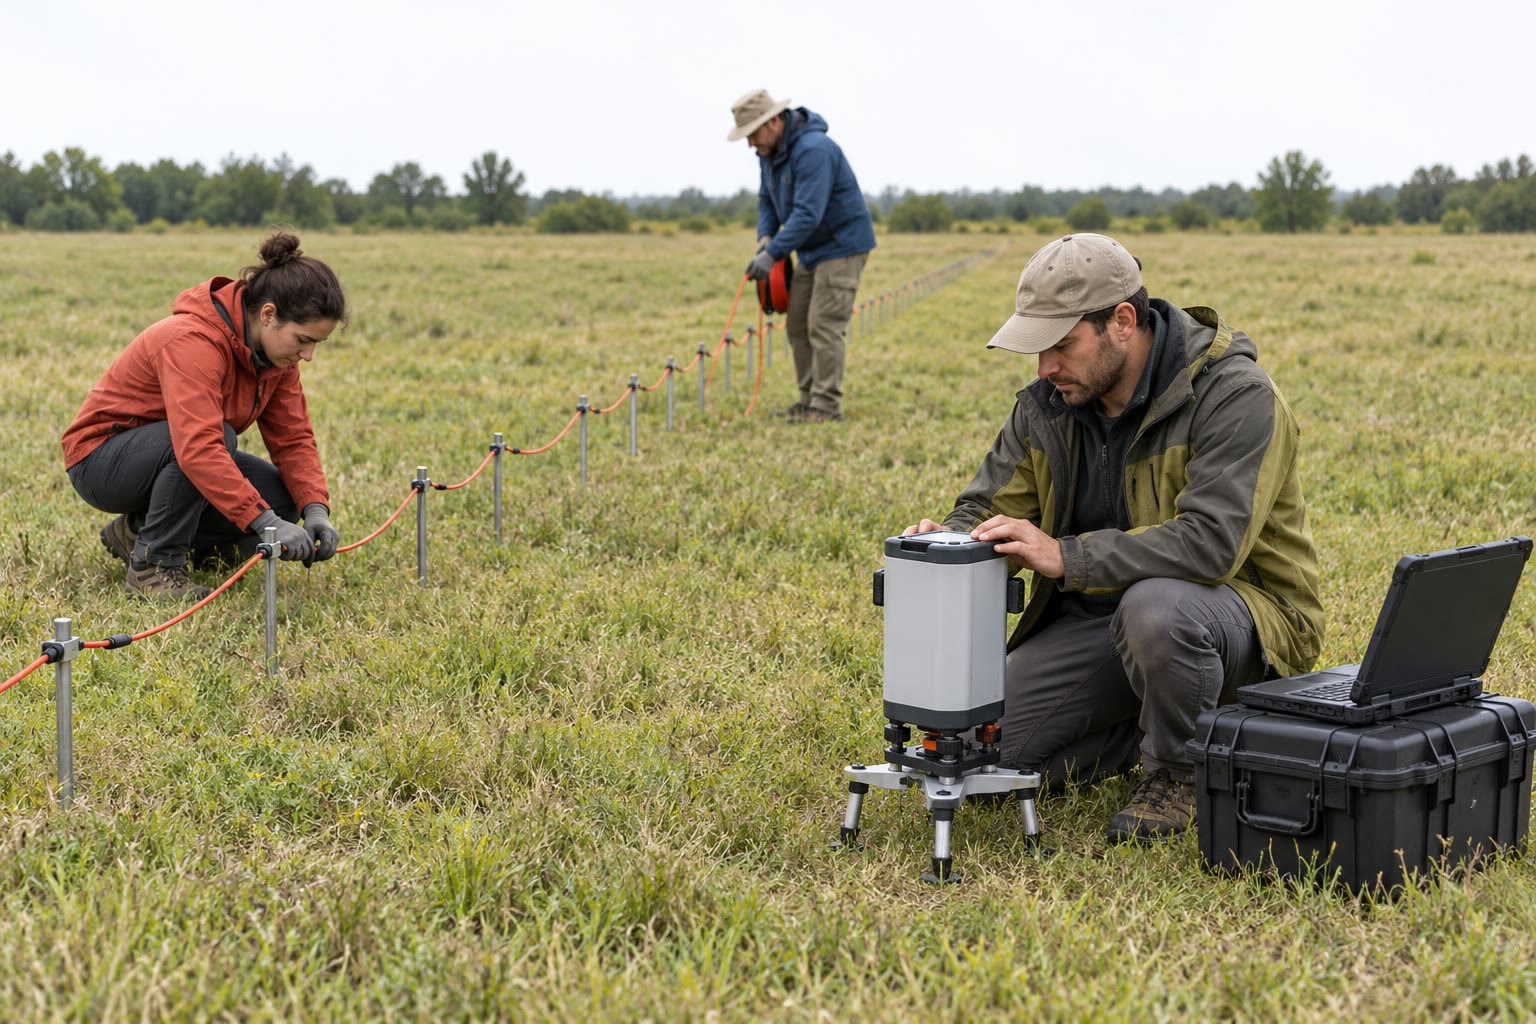
\includegraphics[width=\linewidth]{images/book5/ai/b3-geophysics-crew.jpg}

{\scriptsize Une équipe de géophysiciens déroulant un câble de résistivité, avec un
gravimètre posé sur sa base (illustration générée par IA).}
\end{minipage}
\end{inthefield}

\begin{example}[La campagne de Varden]\label{ex:b3:field-lab-methods-3:varden}
La carte de pesanteur montre une dépression fermée d'environ \qty{-2.3}{\milli\gal},
centrée sur le granite, allongée nord--sud~: le granite clair se prolonge sous la
couverture, et il est le plus long dans cette direction. La dépression s'étend sur
environ \qty{1}{km} à partir de l'affleurement, de sorte que le corps s'élargit
avec la profondeur. Sa demi-largeur donne une première profondeur pour une sphère
équivalente~; des modèles à flanc vertical et à base montrent qu'une base située
entre un et quelques kilomètres de profondeur explique tout aussi bien le pic, à
quelques dixièmes de milligal près, de sorte que la base reste inconnue~: c'est la
non-unicité de la section précédente. Sur le fond de la vallée, au-dessus du granite,
le sondage part de la résistivité d'un gravier sec, plonge là où le courant entre
dans les alluvions saturées d'eau et remonte selon une droite de pente un~: une
couverture conductrice sur un substratum très résistant, le granite, à quelques
mètres de profondeur. Le \omterm{def:b3:field-lab-methods-3:gpr}{géoradar} tiré sur ce même fond montre un écho plat vers
\qty{20}{ns}~: le niveau de la nappe. Quant à la ligne magnétique tracée au travers
du flanc ouest du pli, là où la couverture est épaisse et où les schistes du
socle se trouvent à deux cents mètres environ de profondeur, elle enregistre une
anomalie positive symétrique d'environ \qty{20}{nT} qu'aucune carte n'explique~: un
dyke mafique, riche en magnétite, enfoui sous la couverture~; sa direction le long
du méridien magnétique explique que l'anomalie soit symétrique. Les géophysiciens
le rapportent comme un dyke de dolérite tronqué par la discordance, que la
couverture de la carte dissimule. Le problème du week-end réduit les données de la
campagne.
\end{example}
% ledger: gpg:susceptibility, gpg:resistivity, gpg:gpr-table

\section{Exercices}

\begin{exercise}[$\star$]\label{exo:b3:field-lab-methods-3:1}
(a)~Quelle fraction de $g = \qty{9.81}{m.s^{-2}}$ représente \qty{0.01}{\milli\gal}~?
(b)~De combien faut-il élever un gravimètre pour que sa lecture change
de \qty{0.01}{\milli\gal} sous le seul effet de l'air libre~? (c)~Sous l'effet conjugué
de l'air libre et de Bouguer, avec la masse volumique
\qty{2670}{kg.m^{-3}}~?
\end{exercise}

\begin{exercise}[$\star$]\label{exo:b3:field-lab-methods-3:2}
Une sphère de rayon \qty{50}{m} et de contraste de masse volumique
\qty{+500}{kg.m^{-3}} a son centre à \qty{100}{m} de profondeur. Calculer sa
masse excédentaire, le pic de son anomalie et la demi-largeur $x_{1/2}$.
\end{exercise}

\begin{exercise}[$\star$]\label{exo:b3:field-lab-methods-3:3}
Un dispositif de Wenner d'espacement $a = \qty{10}{m}$ injecte \qty{0.1}{A} et
mesure \qty{0.239}{V}. (a)~Calculer le facteur géométrique et la \omterm{def:b3:field-lab-methods-3:resistivity}{résistivité
apparente}. (b)~Montrer qu'un dispositif de Schlumberger avec $s =
\qty{15}{m}$ et $l = \qty{5}{m}$ a le même facteur géométrique, et expliquer
pourquoi.
\end{exercise}

\begin{exercise}[$\star$]\label{exo:b3:field-lab-methods-3:4}
Le granite a $\varepsilon_r = 5$. (a)~Calculer la vitesse du radar. (b)~Une
fracture se trouve à \qty{10}{m} de profondeur~: calculer le temps double de son
écho. (c)~Avec $\sigma = \qty{1}{mS.m^{-1}}$, calculer la profondeur de peau et la
profondeur utile, soit environ trois profondeurs de peau. (d)~Comparer avec une
argile humide de $\varepsilon_r = 20$ et $\sigma = \qty{10}{mS.m^{-1}}$.
\end{exercise}

\begin{exercise}[$\star\star$]\label{exo:b3:field-lab-methods-3:5}
(a)~Établir l'anomalie d'un long cylindre horizontal de rayon $R$ et de contraste
de masse volumique $\Delta\rho$, dont l'axe se trouve à la profondeur $z$, à partir
de celle d'une masse linéique, et montrer que $z = x_{1/2}$. (b)~Un cylindre et une
sphère donnent le même pic et la même demi-largeur $x_{1/2} = \qty{100}{m}$.
Comparer leurs profondeurs. Quelle interprétation donne le corps le plus profond~?
\end{exercise}

\begin{exercise}[$\star\star$]\label{exo:b3:field-lab-methods-3:6}
L'anomalie de Bouguer du modèle du granite de Varden, échantillonnée tous les
\qty{100}{m} sur une carte de \num{1120} points couvrant $\qty{3.5}{km}
\times \qty{3.2}{km}$, totalise \qty{-438}{\milli\gal}. (a)~Appliquer
la \cref{prop:b3:field-lab-methods-3:gauss} pour estimer le déficit de masse.
(b)~Le déficit de masse du modèle est de \qty{1.74e11}{kg}. Quelle fraction la
carte restitue-t-elle, et où se trouve le reste~?
\end{exercise}

\begin{exercise}[$\star\star$]\label{exo:b3:field-lab-methods-3:7}
(a)~Un dyke mince a son sommet à \qty{30}{m} de profondeur. En utilisant la règle de
trois mesures par demi-largeur, où la demi-largeur est la largeur totale de
l'anomalie à la moitié de son pic, quel espacement de stations lui faut-il~? (b)~Même
question pour un sommet à \qty{220}{m} de profondeur. (c)~Pourquoi une seule campagne
ne peut-elle pas résoudre à la fois un corps superficiel et un corps profond, sauf si
elle est conçue pour le corps superficiel~?
\end{exercise}

\begin{exercise}[$\star\star$]\label{exo:b3:field-lab-methods-3:8}
Un grès saturé d'une eau de résistivité \qty{8}{\ohm\metre} présente une résistivité de
\qty{80}{\ohm\metre}. (a)~Avec $a = 1$ et $m = 2$, calculer sa porosité. (b)~Reprendre
avec $m = 1.8$ et $m = 2.2$. Quel terme de la mesure contrôle l'incertitude sur la
porosité~?
\end{exercise}

\begin{exercise}[$\star\star$]\label{exo:b3:field-lab-methods-3:9}
(a)~Calculer les trois premiers termes de la série à deux couches donnée
par la \cref{prop:b3:field-lab-methods-3:layers} pour $s = 2h_1$ et $k =
\num{0.5}$ et $k = \num{-0.5}$, ainsi que les \omterm{def:b3:field-lab-methods-3:resistivity}{résistivités apparentes}
qu'elles donnent. (b)~Quelles sont les limites de $\rho_a/\rho_1$ pour $s \ll h_1$ et
$s \gg h_1$~? (c)~Quels rapports de résistivités $\rho_2/\rho_1$ correspondent à
$k = \pm 0.5$~?
\end{exercise}

\begin{exercise}[$\star\star\star$]\label{exo:b3:field-lab-methods-3:10}
(a)~Établir le facteur géométrique du dispositif de Wenner à partir
du \cref{thm:b3:field-lab-methods-3:point-source}. (b)~Établir celui du
dispositif de Schlumberger, et montrer que $\rho_a \to 2\pi s^2(-\mathrm{d}V/
\mathrm{d}r)/I$ lorsque $l/s \to 0$. (c)~De combien le facteur approché
$\pi s^2/(2l)$ surestime-t-il le facteur exact lorsque $l = s/10$~?
\end{exercise}

\begin{exercise}[$\star\star\star$]\label{exo:b3:field-lab-methods-3:11}
Une station se trouve à \qty{50}{m} au-dessus de la station de base. Sa lecture est précise à
\qty{0.01}{\milli\gal}, son altitude à \qty{5}{cm}~; la masse volumique du
plateau est incertaine de \qty{100}{kg.m^{-3}}, la \omterm{def:b3:field-lab-methods-3:terrain}{correction de terrain} de
\qty{0.2}{\milli\gal}. (a)~Établir le bilan d'erreurs de son anomalie
de Bouguer. (b)~Quel terme domine, et lequel faudrait-il améliorer pour
détecter une anomalie de \qty{0.1}{\milli\gal}~? (c)~Quel est le total sans
le terme de terrain~?
\end{exercise}

\begin{exercise}[$\star\star\star$]\label{exo:b3:field-lab-methods-3:12}
Cinq mesures de pesanteur le long d'un corps enfoui, en $x = -600$, $-300$, $0$,
$300$ et \qty{600}{m}, valent \num{-0.69}, \num{-2.17}, \num{-4.16},
\num{-2.10} et \qty{-0.73}{\milli\gal}, chacune avec $\sigma =
\qty{0.03}{\milli\gal}$. (a)~Pour des modèles de sphère centrés sous $x = 0$ à des
profondeurs de \num{300}, \num{400} et \qty{500}{m}, choisir la masse qui
ajuste la mesure centrale et calculer l'\omterm{def:b3:field-lab-methods-3:inversion-practice}{écart d'ajustement} $\chi^2$ de chacun. (b)~Quel
modèle ajuste les données dans leurs erreurs~? (c)~Un corps d'une autre
forme pourrait-il ajuster aussi bien~? Qu'est-ce qui trancherait~?
\end{exercise}

\section{Problème~: les corps cachés des Varden Hills}

\begin{problem}[{Problème du week-end --- réduction de la campagne Varden}]
\label{pb:b3:field-lab-methods-3:1}
Utiliser $G = \qty{6.674e-11}{m^3.kg^{-1}.s^{-2}}$, le gradient à
l'air libre \qty{0.3086}{\milli\gal.m^{-1}} et le facteur de Bouguer
\qty{0.1119}{\milli\gal.m^{-1}} (masse volumique \qty{2670}{kg.m^{-3}}).

\medskip\noindent\textbf{Partie I --- Une boucle gravimétrique.} Une boucle sur le
profil gravimétrique donne (lectures en milligals après étalonnage, altitudes
en mètres, temps en heures après 09:00)~:
\begin{center}
\small
\begin{tabular}{lccccc}
\hline
station & base & \qty{3.0}{km} & \qty{3.5}{km} & \qty{4.0}{km} & base \\
\hline
temps & 0 & 0.5 & 0.9 & 1.3 & 2.0 \\
altitude & 176.1 & 149.0 & 145.5 & 158.0 & 176.1 \\
lecture & 2846.512 & 2851.075 & 2850.497 & 2849.392 & 2846.708 \\
\hline
\end{tabular}
\end{center}
\begin{enumerate}
\item Calculer la vitesse de dérive de la boucle.
\item Corriger de la dérive les trois lectures aux stations et les exprimer
  par rapport à la station de base.
\item Appliquer les corrections à l'air libre et de Bouguer pour les
  différences d'altitude, et donner l'anomalie de Bouguer de chaque station par rapport à
  la station de base.
\item La dérive de l'instrument seul était de \qty{0.040}{\milli\gal.h^{-1}}.
  Qu'est-ce qui a causé le reste de la variation à la station de base, et pourquoi
  elle pouvait être éliminée avec la dérive~?
\item Le modèle dont proviennent les lectures donne les trois anomalies
  par rapport à la station de base~: \num{-0.825}, \num{-2.131} et
  \qty{-0.825}{\milli\gal}. Calculer les erreurs de la réduction. Les
  altitudes du tableau sont arrondies à \qty{0.1}{m}~: quelle erreur cet
  arrondi peut-il introduire, et explique-t-il les erreurs~?
\item Quelle précision sur l'altitude garde l'anomalie réduite dans
  \qty{0.01}{\milli\gal}~? Pourquoi les manuels de campagne exigent-ils
  \qty{3.3}{cm}, une valeur plus serrée~?
\end{enumerate}

\medskip\noindent\textbf{Partie II --- L'anomalie du granite.} Le long du
profil, l'anomalie présente son minimum, \qty{-2.293}{\milli\gal}, en
$x = \qty{3.50}{km}$, et passe par la moitié de cette valeur en $x = 3.048$ et
\qty{3.952}{km}. Le modèle du granite présente un contraste de masse volumique de
\qty{-130}{kg.m^{-3}}, et le sol au centre se situe à \qty{145.5}{m}
au-dessus du niveau de la mer.
\begin{enumerate}[resume]
\item Calculer la demi-largeur $x_{1/2}$ et la profondeur du centre de
  la sphère équivalente.
\item Calculer le déficit de masse de cette sphère, et son rayon pour le
  contraste de masse volumique du granite. Qu'y a-t-il de surprenant dans ce résultat~?
\item Le centre de masse du modèle se situe à \qty{864}{m} sous le sol et son
  déficit de masse vaut \qty{1.74e11}{kg}. Pourquoi la règle de la demi-largeur donne-t-elle un
  corps moins profond et moins lourd~?
\item Un cylindre vertical de même section que le granite au
  niveau de la discordance a un rayon de \qty{461}{m}. Calculer son anomalie sur l'axe
  pour un sommet au niveau du sol et un plancher à \qty{1645}{m} de profondeur, et pour une
  profondeur illimitée.
\item Trouver, par essais ou par résolution, la profondeur du plancher pour laquelle ce
  cylindre donne l'anomalie observée de \qty{-2.29}{\milli\gal}.
\item Calculer l'anomalie du cylindre avec son sommet à \qty{6}{m} de profondeur
  (plancher à \qty{1645}{m}). La gravimétrie permet-elle de dire si le granite atteint
  la surface sous les alluvions~?
\end{enumerate}

\medskip\noindent\textbf{Partie III --- Le fond de la vallée.} Le sondage Schlumberger
effectué sur le fond au-dessus du granite donne (demi-écartement $s$ en
mètres, $\rho_a$ en \unit{\ohm\metre})~:
\begin{center}
\small
\begin{tabular}{lcccccccc}
\hline
$s$ & 1 & 2 & 4 & 6 & 10 & 20 & 30 & 40 \\
$\rho_a$ & 577 & 526 & 387 & 350 & 449 & 821 & 1309 & 1684 \\
\hline
\end{tabular}
\end{center}
Sur un profil radar le long de ce même fond, une canalisation donne une hyperbole dont
le sommet est à \qty{10.7}{ns} et le temps est de \qty{17.1}{ns} à \qty{1}{m}
de côté~; un écho plat arrive à \qty{20.0}{ns}.
\begin{enumerate}[resume]
\item Pour $s = \qty{20}{m}$, MN mesurait \qty{2}{m} de long et le courant
  \qty{50}{mA}. Calculer le facteur géométrique et la tension mesurée.
\item Calculer la vitesse radar, la permittivité relative des
  alluvions et la profondeur de la canalisation.
\item L'écho plat correspond au niveau de la nappe. Quelle est sa profondeur~?
\item Estimer la conductance $S$ des alluvions à partir des lectures aux
  20, 30 et \qty{40}{m}.
\item Les alluvions sèches ont \qty{600}{\ohm\metre} et les alluvions saturées
  \qty{222}{\ohm\metre}. Calculer l'épaisseur des alluvions saturées et la
  profondeur du sommet du granite. L'estimation est-elle haute
  ou basse, et pourquoi~?
\item L'eau souterraine a \qty{20}{\ohm\metre}. Calculer la porosité des
  alluvions par la \omterm{prop:b3:field-lab-methods-3:archie}{loi d'Archie} avec $m = 2$, et l'intervalle pour $m$
  entre \num{1.3} et \num{2.8}.
\end{enumerate}

\medskip\noindent\textbf{Partie IV --- La ligne magnétique.} La ligne court
vers l'est à partir de $x = \qty{1.70}{km}$, une station tous les \qty{50}{m} et
toutes les deux minutes~; la station de base a enregistré aux mêmes minutes. Les
lectures, moins \qty{48000}{nT}, sont~:
\begin{center}
\small
\setlength{\tabcolsep}{3.5pt}
\begin{tabular}{lccccccccccc}
\hline
$x$ (km) & 1.70 & 1.75 & 1.80 & 1.85 & 1.90 & 1.95 & 2.00 & 2.05 & 2.10 & 2.15 & 2.20 \\
ligne & 3.4 & 4.8 & 6.3 & 8.1 & 10.3 & 12.8 & 15.8 & 19.2 & 22.9 & 26.2 & 28.0 \\
base & 0.0 & 0.7 & 1.5 & 2.2 & 2.9 & 3.6 & 4.3 & 5.0 & 5.7 & 6.4 & 7.0 \\
\hline
$x$ (km) & 2.25 & 2.30 & 2.35 & 2.40 & 2.45 & 2.50 & 2.55 & 2.60 & 2.65 & 2.70 & \\
ligne & 27.7 & 25.8 & 23.3 & 20.9 & 19.0 & 17.6 & 16.6 & 15.9 & 15.5 & 15.2 & \\
base & 7.6 & 8.2 & 8.8 & 9.4 & 9.9 & 10.4 & 10.9 & 11.3 & 11.7 & 12.1 & \\
\hline
\end{tabular}
\end{center}
Le champ principal est \qty{48000}{nT}, incliné à \ang{65}.
\begin{enumerate}[resume]
\item Appliquer la \omterm{def:b3:field-lab-methods-3:magnetic}{correction diurne} et donner l'anomalie corrigée à
  chaque station.
\item Montrer que, sans la correction, l'anomalie ne descend jamais à
  la moitié de son maximum du côté est.
\item Localiser le maximum et les deux points où l'anomalie corrigée vaut
  la moitié du maximum, par interpolation linéaire, et calculer la demi-largeur.
\item L'anomalie est symétrique. Que dit cela de la direction
  du corps, et quel type de corps la règle de la demi-largeur suppose-t-elle~?
\item Calculer le produit $\kappa t$ de la susceptibilité et de l'épaisseur.
  Si le filon est une dolérite de susceptibilité \num{0.03}, quelle
  est son épaisseur~?
\item Les stations étaient-elles assez rapprochées~?
\item Donner la profondeur du toit du filon enfoui sous le sol, à
  la dizaine de mètres près, et la comparer à la profondeur de la
  discordance du modèle géologique de la région, \qty{222}{m} en ce
  point.
\end{enumerate}
\end{problem}
% ledger: gpg:grav-survey, gpg:mag-field, keys:archie
